\chapter{Chapter3}
This document contains commonly used essential templates to write a
\LaTeX\ document. This document is to be used along with the files and
folders provided. Writing a \LaTeX\ document is very simple.  Often
students need only very simple constructs.  This document shows
certain essential features that almost all technical report writing
requires. Please consult the PDF file for the output of the document,
and then look at the corresponding \LaTeX\ file to reproduce it.  The
document illustrates the following constructs
% Commands to include a figure:
%\begin{figure}
%\includegraphics[width=\textwidth]{your-figure's-file-name}
%\caption{\label{fig:your-figure}Caption goes here.}
%\end{figure}

\begin{itemize}
\item Unnumbered and numbered Lists
\item Equations
\item Defining short macros for frequently used symbols
\item Bibliography
\item Figures
\item Tables
\end{itemize}
\begin{figure}[tbp]
  \centering
    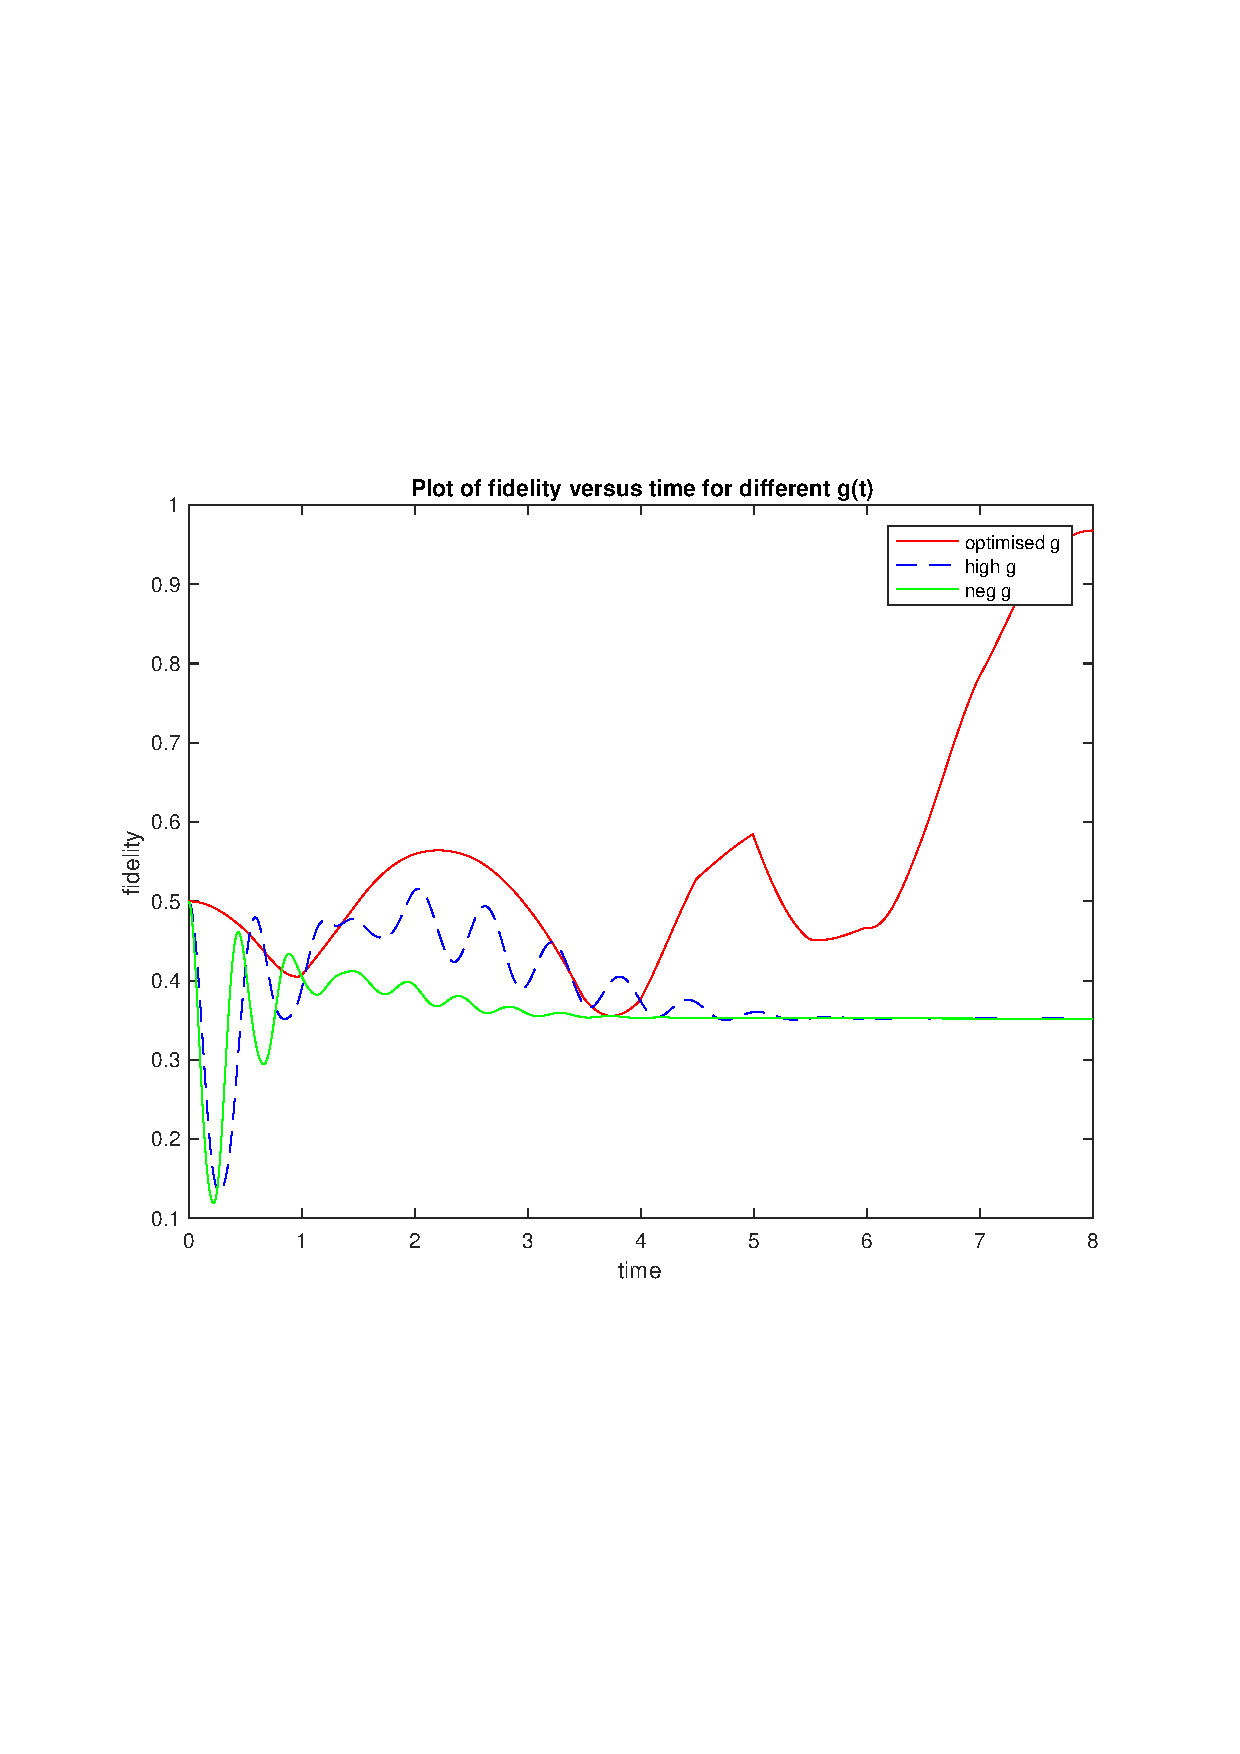
\includegraphics[width=1.0\textwidth]{gvary7}
    \caption[Process flow sheet]{varying g of the
      experimental setup. The caption of the figure goes here. A
      shorter caption can be written in square brackets to identify it
      in the list of figures.}
    \label{fig:gvary7} 
\end{figure}